% !TEX TS-program = XeLaTeX
% use the following command:
% all document files must be coded in UTF-8
\documentclass[spanish]{textolivre}
% build HTML with: make4ht -e build.lua -c textolivre.cfg -x -u article "fn-in,svg,pic-align"

\journalname{Texto Livre}
\thevolume{16}
%\thenumber{1} % old template
\theyear{2023}
\receiveddate{\DTMdisplaydate{2021}{11}{15}{-1}} % YYYY MM DD
\accepteddate{\DTMdisplaydate{2022}{3}{7}{-1}}
\publisheddate{\DTMdisplaydate{2022}{10}{31}{-1}}
\corrauthor{José Antonio Cordón García}
\articledoi{10.1590/1983-3652.2023.37067}
%\articleid{NNNN} % if the article ID is not the last 5 numbers of its DOI, provide it using \articleid{} commmand 
% list of available sesscions in the journal: articles, dossier, reports, essays, reviews, interviews, editorial
\articlesessionname{dossier}
\runningauthor{Cordón García y Muñoz Rico} 
%\editorname{Leonardo Araújo} % old template
\sectioneditorname{Hugo Heredia Ponce}
\layouteditorname{Daniervelin Pereira}

\title{La socialización de la lectura y la escritura: fandom, redes y visibilidad editorial}
\othertitle{A socialização da leitura e da escrita: fandom, redes e visibilidade editorial}
\othertitle{The socialization of reading and writing: fandom, networks and publishing visibility}
% if there is a third language title, add here:
%\othertitle{Artikelvorlage zur Einreichung beim Texto Livre Journal}

\author[1]{José Antonio Cordón García~\orcid{0000-0002-8569-9417}\thanks{Email: \href{mailto:jcordon@usal.es}{jcordon@usal.es}}}
\author[2]{María Muñoz Rico~\orcid{0000-0002-7333-4832}\thanks{Email: \href{mailto:ricom@usal.es}{ricom@usal.es}}}
\affil[1]{Universidad de Salamanca, Facultad de Traducción y Documentación, Departamento de Biblioteconomía y Documentación, Salamanca, España.}
\affil[2]{Universidad de Salamanca, Grupo E-lectra de Investigación, Instituto de Estudios Medievales, Renacentistas y de Humanidades Digitales (IEMYRhd), Salamanca, España.}

\addbibresource{article.bib}
% use biber instead of bibtex
% $ biber article

% used to create dummy text for the template file
\definecolor{dark-gray}{gray}{0.35} % color used to display dummy texts
\usepackage{lipsum}
\SetLipsumParListSurrounders{\colorlet{oldcolor}{.}\color{dark-gray}}{\color{oldcolor}}

% used here only to provide the XeLaTeX and BibTeX logos
\usepackage{hologo}

% if you use multirows in a table, include the multirow package
\usepackage{multirow}

% provides sidewaysfigure environment
\usepackage{rotating}

% CUSTOM EPIGRAPH - BEGIN 
%%% https://tex.stackexchange.com/questions/193178/specific-epigraph-style
\usepackage{epigraph}
\renewcommand\textflush{flushright}
\makeatletter
\newlength\epitextskip
\pretocmd{\@epitext}{\em}{}{}
\apptocmd{\@epitext}{\em}{}{}
\patchcmd{\epigraph}{\@epitext{#1}\\}{\@epitext{#1}\\[\epitextskip]}{}{}
\makeatother
\setlength\epigraphrule{0pt}
\setlength\epitextskip{0.5ex}
\setlength\epigraphwidth{.7\textwidth}
% CUSTOM EPIGRAPH - END

% LANGUAGE - BEGIN
% ARABIC
% for languages that use special fonts, you must provide the typeface that will be used
% \setotherlanguage{arabic}
% \newfontfamily\arabicfont[Script=Arabic]{Amiri}
% \newfontfamily\arabicfontsf[Script=Arabic]{Amiri}
% \newfontfamily\arabicfonttt[Script=Arabic]{Amiri}
%
% in the article, to add arabic text use: \textlang{arabic}{ ... }
%
% RUSSIAN
% for russian text we also need to define fonts with support for Cyrillic script
% \usepackage{fontspec}
% \setotherlanguage{russian}
% \newfontfamily\cyrillicfont{Times New Roman}
% \newfontfamily\cyrillicfontsf{Times New Roman}[Script=Cyrillic]
% \newfontfamily\cyrillicfonttt{Times New Roman}[Script=Cyrillic]
%
% in the text use \begin{russian} ... \end{russian}
% LANGUAGE - END

% EMOJIS - BEGIN
% to use emoticons in your manuscript
% https://stackoverflow.com/questions/190145/how-to-insert-emoticons-in-latex/57076064
% using font Symbola, which has full support
% the font may be downloaded at:
% https://dn-works.com/ufas/
% add to preamble:
% \newfontfamily\Symbola{Symbola}
% in the text use:
% {\Symbola }
% EMOJIS - END

% LABEL REFERENCE TO DESCRIPTIVE LIST - BEGIN
% reference itens in a descriptive list using their labels instead of numbers
% insert the code below in the preambule:
%\makeatletter
%\let\orgdescriptionlabel\descriptionlabel
%\renewcommand*{\descriptionlabel}[1]{%
%  \let\orglabel\label
%  \let\label\@gobble
%  \phantomsection
%  \edef\@currentlabel{#1\unskip}%
%  \let\label\orglabel
%  \orgdescriptionlabel{#1}%
%}
%\makeatother
%
% in your document, use as illustraded here:
%\begin{description}
%  \item[first\label{itm1}] this is only an example;
%  % ...  add more items
%\end{description}
% LABEL REFERENCE TO DESCRIPTIVE LIST - END


% add line numbers for submission
%\usepackage{lineno}
%\linenumbers

\begin{document}
\maketitle

\begin{polyabstract}
\begin{abstract}
La lectura ha experimentado cambios significativos en la última década, caracterizados por la modificación del comportamiento del público lector, así como por las formas de acceso y consumo. Uno de los aspectos más significativos ha sido el papel cada vez más activo que han recibido los lectores en el proceso de recepción, cobrando un mayor protagonismo gracias a las posibilidades de intervención en forma de comentarios, recomendaciones, e intercambio de información de diversa naturaleza entre ellos. Pero también a su organización en redes de intereses a partir de un texto o un autor, constituyendo grupos de fan, que no sólo dialogan y participan y promueven actos de promoción y reivindicación de tramas y escenarios, sino que alimentan el \textit{corpus} mediante creaciones propias o traducciones anticipadas. Con todo ello se incrementan los niveles de visibilidad de las obras y autores, favoreciendo su difusión y coadyuvando indirectamente a la actividad editorial, que ha modificado parte de sus tareas promocionales amparada en estos nuevos escenarios. Se analiza en el artículo la incidencia de estos fenómenos desde el punto de vista de las métricas en bases de datos y desde el influjo en la actividad creativa y editorial.

\keywords{Fandon \sep Fanfitions \sep Lectura social \sep Redes Sociales \sep Visibilidad editorial}
\end{abstract}

\begin{portuguese}
\begin{abstract}
A leitura passou por mudanças significativas na última década, caracterizada pela modificação do comportamento do público leitor, bem como pelas formas de acesso e consumo. Um dos aspectos mais significativos tem sido o papel cada vez mais ativo que os leitores têm recebido no processo de recepção, ganhando maior destaque graças às possibilidades de intervenção na troca de informações de natureza diversa entre eles, além de interações na forma de comentários e recomendações. Sobretudo, é notória sua organização em redes de interesses a partir de um texto ou de um autor, constituindo grupos de fãs, que não apenas dialogam, participam, promovem atos de promoção e reivindicação de enredos e cenários, mas também alimentam o \textit{corpus} por meio de suas próprias criações ou traduções antecipadas. Com tudo isso, aumentam-se os níveis de visibilidade das obras e autores, favorecendo sua difusão e contribuindo indiretamente para a atividade editorial, que modificou parte de suas tarefas promocionais protegidas por esses novos cenários. A incidência desses fenômenos é analisada no artigo do ponto de vista das métricas em bancos de dados e da influência na atividade criativa e editorial.

\keywords{Fandom \sep Fanfictions \sep Leitura social \sep Redes Sociais \sep Visibilidade editorial}
\end{abstract}
\end{portuguese}

\begin{english}
\begin{abstract}
Reading practices have undergone  meaningful transformations in recent years, characterised by changes in the behaviour of the reading public, as well as in the manner in which material is accessed and consumed. One of the most significant developments has been the increasingly active role played by readers in the reception process. Readers now have more of an influence owing to opportunities to intervene in the form of comments, recommendations, and exchanges of various kinds of information among readers. At the same time, readers are also organised into interest groups based on a text or an author, forming fan clubs. Through this network, readers not only discuss, participate, and initiate events to promote plot and scene development, but also feed the corpus through their own creations or anticipated translations. As a result, the visibility levels of works and authors are increased, favouring their dissemination and indirectly contributing to the publishing process, which has shifted part of its promotional work in light of this new situation. This article analyses the incidence of these processes from the point of view of both quantitative and qualitative parameters provided by different databases, as well as their impact on creative and editorial activities.

\keywords{Fandom \sep Fanfictions \sep Publishing visibility \sep  Social networks \sep Social Reading}
\end{abstract}
\end{english}
% if there is another abstract, insert it here using the same scheme
\end{polyabstract}

\section{Introducción}\label{sec-intro}
Los cambios en el comportamiento del público lector y la importancia creciente de las redes sociales han erigido a estas en uno de los factores fundamentales para la promoción y venta de los libros, afectando tanto a autores y editoriales, obligados a trabajar sobre las obras en sus distintas fases de elaboración, garantizando su presencia en la red, pero también le ha conferido un gran poder de articulación del mercado y de orientación de las decisiones de compra a los lectores, que a través de opiniones, comentarios, recomendaciones y creación de clubes de apoyo, a un autor, un personaje o una obra, condicionan el balance de resultados y el posicionamiento de estos elementos en el mercado \cite{faggiolani_redes_2019}.

Este fenómeno está alimentado por dos tendencias concurrentes. Por una parte, por la progresiva incorporación de lectores digitales jóvenes que prestan más atención a la temática y al autor que a la editorial, como se puede apreciar en los diferentes estudios sobre consumo en las series estadísticas publicadas en los diferentes países. Por otra, por la importancia de las redes sociales en los sistemas de recomendación de contenidos, que se han configurado como un factor de influencia cada vez más poderoso \cite{pianzola_wattpad_2020,pianzola_digital_2021}. 

Las editoriales y los autores cada vez son más deudores de su presencia en las redes sociales, obligados a desarrollar estrategias de visibilidad agresiva que provoquen la fidelización del lector, una característica propia de las industrias culturales digitales \cite{duhigg_power_2012}. Esta hipervisibilidad, muchas veces motivada por contrato, es aún más importante en el caso de los autores autopublicados, responsables únicos de la difusión y distribución de su obra. Este fenómeno ha provocado que la participación de los autores en todo tipo de redes sociales, mediante páginas de sus obras, páginas personales en Facebook, sitios web propios, cuentas en Twitter, en Goodreads, etc, forme parte del elenco de rutinas que han de desarrollar como privativas de su oficio \cite{lluch_claves_2018}. Esto también ha provocado que la línea de separación entre la promoción y el spam sea cada vez más débil.  

El problema es el mantenimiento del equilibrio cuando la oferta crece exponencialmente y los espacios de exposición, físicos y digitales, la abocan a la invisibilidad sin este tipo de intervenciones o de intrusiones en los huecos del mercado digital. Los autores son más dependientes de los lectores que nunca, y necesitan del marketing viral de sus comentarios y anotaciones para su supervivencia, de ahí que fuercen la presencia de su persona y de sus obras en cuantos lugares disponibles puedan encontrar, a veces con efectos completamente contraproducentes \cite{munoz_rico_bestsellers_2022}.

En un ensayo premonitorio, \textcite{stein_taxonomy_2010}, acuñó el término de “Social Book” para referirse a las obras que facilitan el intercambio de información, la colaboración entre los lectores, la incorporación de novedades, el anotado y la integración en redes de todo tipo. Para Stein, lo Social se refiere tanto a la interacción con el otro como a la conversación. Además, al leer socialmente, se etiqueta la página en varios niveles, como marcas gráficas, notas y comentarios. Social también alude al acceso a los comentarios de todos los que leen en el sistema. \textcite{stein_taxonomy_2010} propone una taxonomía de la lectura social que iría de lo informal a lo formal, desde el libro a las “afueras del libro”. Pero la lectura social reviste otros muchos componentes cada vez más involucrados en la idiosincrasia del libro como producto, inherentes a tanto a su desarrollo comercial como receptivo \cite{cruces_villalobos_como_2017}.

La capacidad de proyección de los comentarios y aprobaciones en la red está implícita en los movimientos de editores y grupos de comunicación para potenciar la presencia social de los autores. Los responsables de marketing de las casas editoriales, y de cualquier empresa en la red, saben que las opiniones positivas influyen poderosamente en Internet. En un estudio desarrollado por investigadores de varias universidades, tomando como referencia los comentarios escritos en Facebook y Reddit, se concluye que la influencia social negativa tiende a corregir las calificaciones a la baja, mientras que la probabilidad de que un comentario positivo arrastre a otro es del 32~\%. En este mismo estudio se demuestra que los “me gusta” acarrean una acumulación de un 25~\% más de reacciones favorables \cite{cordon-garcia_evolution_2019}. 

El compromiso y la implicación de los lectores en los sistemas de recomendación y valoración de las obras no es más que otra vertiente de esa sobreexposición del “yo” en la Red que, como señala \textcite{zafra_entusiasmo:_2017}, forma parte de un sistema de apropiación del entusiasmo canibalizado por las redes sociales que lo gestionan en beneficio de oscuras previsiones algorítmicas. Pero el fenómeno reviste otra vertiente relacionada con los procesos de exposición y potenciación de la visibilidad editorial y autoral, en la medida en que la viralización de contenidos, de forma breve expandida, favorece la extensión de mensajes, implícitamente publicitarios, en las sinuosidades de los nichos reticulares.

De ahí la importancia que han cobrado para muchas editoriales los clubs de seguidores organizados en torno a un autor o una obra \cite{cruz_martin_fenomeno_2016}. Se trata de redes de lectores interesados en la replicación, intercambio de información y creación de tramas en torno a los temas o personajes que tienden a difundir la misma \cite{coppa_fanfiction_2017}, y a crear situaciones de memoria participativa \cite{potts_participatory_2018} gracias a las interacciones que se producen no solo con las obras, sino entre los propios implicados en las redes. \textcite{rodriguez_marcos_21_2019} que la literatura busca lectores y la industria literaria, fans; es decir, masas de fieles que esperan cada año el libro de su autor favorito y que aseguran que las cuentas cuadran. Son interesantes al respecto los términos Canon, Fanom y Fandom, para referirse: el primero a las obras originales, el segundo a las generadas a partir de las originales y el tercero a toda la comunidad \cite{scolari_narrativas_2013,chartier_cultura_2019}.

\section{Objetivos y Método}\label{sec-normas}
Los objetivos de este artículo son, básicamente dos:
\begin{enumerate}[label=\alph*.]
    \item Estudio de la visibilidad científica del fenómeno Fandom en el marco de los procesos de socialización de la lectura.
    \item Análisis y reflexión de lo que este representa desde el punto de vista de la difuminación de las estructuras del campo editorial, así como la aparición de nuevas figuras de autoría y nuevas actitudes en la recepción.
\end{enumerate}

Para el desarrollo del primer objetivo se han seleccionado las dos bases de datos multidisciplinares e internacionales más importantes, a nivel internacional, existentes en la actualidad: Web of Science, y Scopus que, además de ofrecer información bibliográfica, ofrecen métricas y prestaciones de análisis complementarias imprescindibles para contextualizar la visibilidad de la producción científica. En el análisis de la base de datos Wos se han tenido en cuenta tanto las publicaciones de la web principal como las registradas en Emerging Citation Sources (ECS), que supuso una ampliación considerable del círculo restringido de revistas con que contaba la base de datos, motivado principalmente por la competencia generada desde otros sistemas, cuyas métricas implicaban coberturas mayores \cite{somoza-fernandez_journal_2018,de_filippo_is_2020,butt_bibliometric_2021}.

Por otra parte, se han explorado tres bases de datos especializadas, de carácter internacional, pertenecientes al ámbito de las Humanidades y de las Ciencias Sociales: Literatura on line, MLA International Bibliography y Social Science Database. La elección de estas tres bases de datos se ha efectuado en virtud de su conexión con el tema estudiado. Para la elección de las bases de datos se ha tenido en cuenta el metaanálisis desarrollado por \textcite{vuotto_fortalezas_2020}, en el que categorizan y evalúan algunas de las principales bases de datos internacionales.

Para las búsquedas bibliográficas se han empleado los términos Fandom, Fans, Culture, Publishing, Social Reading, Social Network, Writing, Self-Publishing, Authorship. Se han efectuado búsquedas en los campos Título, Topic y Abstract. Las búsquedas se han restringido tipológicamente a los artículos científicos y monografías, para comprobar la representatividad de la literatura científica en cada una de las bases de datos. Igualmente se han efectuado restricciones cronológicas a la producción científica entre los años 2012 y 2021. 

En las bases de datos WOS y Scopus se han empleado las herramientas analíticas que proporciona el sistema con objeto de poder cotejar el grado de productividad e impacto por autores, áreas de conocimiento, años, tipologías documentales y disponibilidad de los recursos, a fin de poder caracterizar los resultados. Igualmente se han utilizado las herramientas de análisis y representación gráfica de las citas, cuya evolución constituye un indicador del impacto y proyección de la investigación sobre un tema en las áreas disciplinares afectadas.

Las estrategias de búsqueda desarrolladas, según los criterios descritos más arriba, se han adaptado a cada una de las bases de datos, cuyas interfaces gráficas difieren, así como sus posibilidades de gestión terminológica. 

Finalmente, para homogeneizar los resultados, facilitar las citas y articular un sistema unificado de registros, se ha empleado la exportación de registro, directa desde la base de datos, o indirecta como archivo Ris, al gestor Refworks que, gracias a su integración con los procesadores de textos permite operativizar la información bibliográfica con la normalización requerida.
	
Para el desarrollo del segundo objetivo, además de analizar los resultados obtenidos en las bases de datos, se han explorado las publicaciones más significativas sobre el tema, tanto a nivel nacional como internacional, realizando un examen crítico de las mismas.

\section{Resultados}\label{sec-conduta}

\subsection{La evolución de la literatura científica}
La evolución de los estudios sobre el fenómeno Fandom y los elementos asociados a esta cuestión evidencia una progresión constante en la literatura científica, muestra del interés creciente que la socialización de los comportamientos culturales entre los sectores de población más alfabetizados digitalmente. 

\begin{table}[h!]
\footnotesize
\begin{threeparttable}
\caption{Resultados de las búsquedas en bases de datos.}
\label{tab01}
\centering
\begin{tabular}{p{2cm} p{1.5cm} p{2.7cm} p{2.7cm} p{2cm} p{1.3cm}}
\toprule
\multicolumn{6}{c}{Resultados en bases de datos de contribuciones sobre el campo de la Fanfictions} \\
Base de datos & Resultados globales & Tipologías temáticas & Tipologías documentales & Evolución cronológica & Acceso abierto  \\
\midrule
Scopus & 1879 & Social Sciences: 1366, Art and Humanities: 708 & Artículos: 1266, Capítulos libros: 299, Libros: 77 & 2012:72, 2021:250 & 374  \\
WOS & 2347 & Social Sciences: 1593, Art and Humanities: 929 & Artículos: 2016, Libros: 286, Artículos de revisión: 160 & 2012:81, 2021: 240 & 411 \\
MLA INTERNATIONAL BIBLIOGRAPHY & 938 & Art and Humanities: 938 & Artículos: 512, Capítulos libros: 286, Libros: 87, Tesis: 27 & 2012:42, 2021: 63 & 144 \\
Literature online & 1305 & Art and Humanities: 1305 & Artículos: 749, Revisiones: 350, Libros: 50 & 2012:70, 2021: 155 & 90 \\
Social Science Database & 1597 & Comunicación: 228, Antropología: 330 , Redes sociales: 320 & Artículos: 920, Libros: 166, Tesis: 366 & 2012:88, 2021: 192 & 1413 \\
\bottomrule
\end{tabular}
\source{Elaboración propia.}
\end{threeparttable}
\end{table}

La \Cref{tab01} resumen de los resultados en las bases de datos evidencia una producción científica abundante sobre la materia, sobre todo en el ámbito de las Humanidades y las Ciencias Sociales. 

La abundante producción de monografías sobre el tema constituye una muestra de la existencia de un interés que sobrepasa a la revista especializada para profundizar en los diferentes aspectos y perspectivas que reviste el fenómeno Fandom. Esta importancia de la monografía académica se complementa con la existencia de numerosos capítulos de libro en obras colectivas y el desarrollo de tesis doctorales y trabajos de doctorado que, por ejemplo, en el caso de Social Science Database alcanzan las 366 contribuciones. La relevancia de las monografías y de los capítulos de libro reviste cierta singularidad, pues la tendencia general es a la presencia casi exclusiva de artículos científicos, con una existencia testimonial de los libros cuyo carácter de centralidad en la comunicación científica ha ido declinando con el tiempo, en benefició de otras formas comunicativas \cite{cordon-garcia_publishing_2022,cordon-garcia_evolution_2019}. Esta circunstancia identifica una de las fortalezas de la investigación en este ámbito pues, sin desatender la literatura científica de urgencia, en términos editoriales, recoge una gran cantidad de reflexiones de carácter más profundo y extenso, promoviendo con ello formas de pensamiento más perdurables en el tiempo. 

La evolución cronológica de las publicaciones evidencia una progresión entre las fechas que se han tomado como referencia, 2012 a 2021, por tomar un periodo de diez años. En todos los casos se puede apreciar un incremento en el número de registros.

Tan significativa como la evolución de las contribuciones es la de las citas sobre las mismas, muestra del interés suscitado entre la comunidad científica, reflejado en las menciones que figuran en la literatura científica. A través de los datos aportados por el análisis realizado en Wos y Scopus se puede apreciar cómo ha existido a lo largo del tiempo una correlación entre publicaciones y citas, de tal manera que las segundas se han ido incrementando sobre todo en los últimos cinco años de manera significativa. De hecho, las citas han experimentado un incremento de 220~\% en el periodo comprendido entre 2017-21, con respecto al de 2012-2016 (\Cref{fig01}). 

\begin{figure}[htbp]
 \centering
 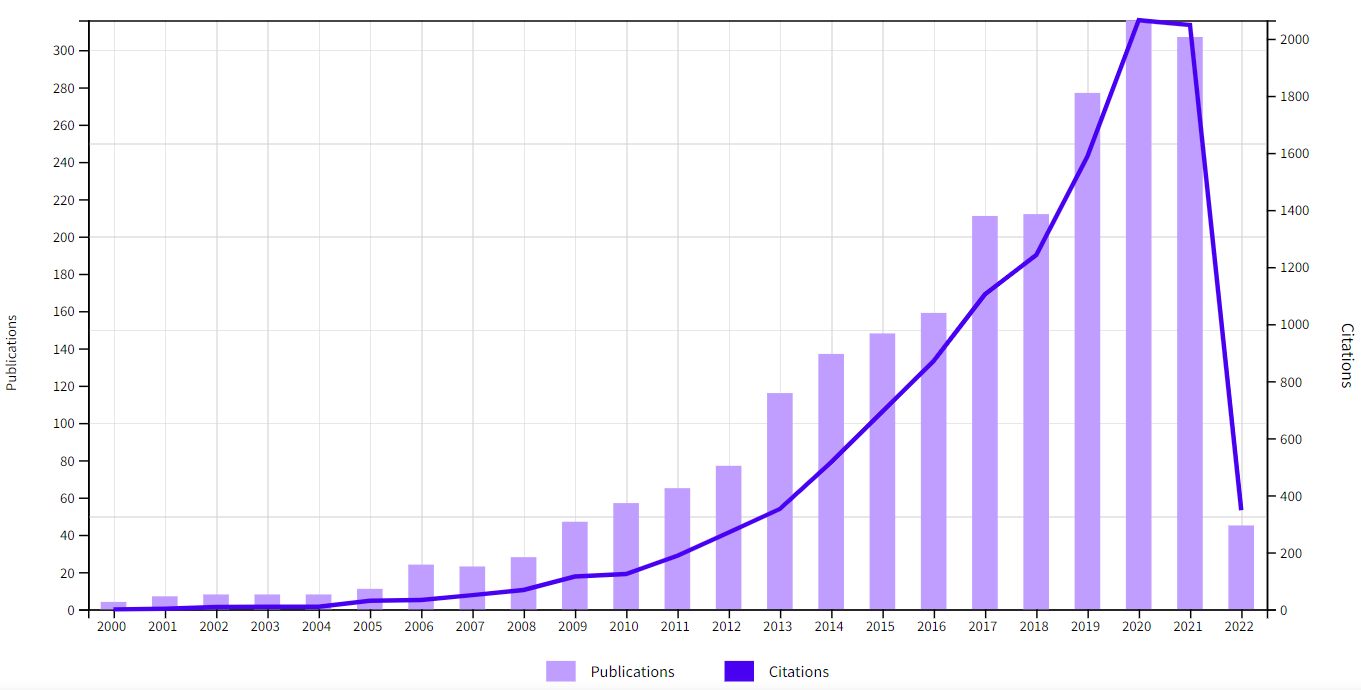
\includegraphics[width=0.85\textwidth]{Fig1.png}
 \caption{Evolución de la producción bibliográfica y la citación sobre el Fandom.}
 \label{fig01}
 \source{Elaboración propia.}
\end{figure}

Los perfiles del gráfico de citas obtenido en la base de datos de la Web of Science a partir de las búsquedas combinadas citadas anteriormente, ilustra la emergencia de la investigación del fenómeno a partir de los inicios del siglo XXI. Aunque previamente el tema había aparecido en la literatura científica, lo había hecho de manera esporádica y sin la regularidad que cobra en el nuevo siglo. Como se puede apreciar en la imagen existe una correlación clara entre producción e impacto, aunque la producción crece de una manera aritmética y las citas de manera exponencial. En paralelo con el incremento en los procesos de citación es preciso señalar como, a partir de 2013, también se incrementan los artículos de revisión de la literatura científica sobre el tema, sobrepasando el centenar. Bajo el paraguas de la revisión sistemática de la literatura (RSL) se encuentran una gran cantidad de fuentes terciarias, cuya presencia en cualquier investigación científica representa un indicador relevante de la entidad de esta \cite{cordon_garcia_nuevas_2016,gomez_diaz_fuentes_2017}. El hecho de contar con numerosos metaanálisis normalmente muy estructurados y bien secuenciados \cite{tricco_prisma_2018}, representa una garantía de solvencia sobre la solidez de un tema de investigación.

\subsection{Las nuevas formas de autoría: la difuminación del campo editorial}\label{sec-fmt-manuscrito}
Los datos evidencian la consolidación de un fenómeno que afecta al polo de la producción escrita, por cuanto esta se multiplica exponencialmente en el ámbito digital, pero con la particularidad de escapar de los límites de lo que \textcite{bourdieu_reglas_2018} había caracterizado como campo editorial. Se trataría de escrituras denominadas por Vicente Luis Mora como creaciones a la intemperie \cite{mora_escritura_2021}, en su intento de trazar una fenomenografía de la escritura digital contemporánea, literaria o no. El concepto de Escritura a la Intemperie es una feliz conceptualización de prácticas y fenómenos muy diversificados, que afectan a toda la cadena del libro digital, desde la autoría a la recepción, cuyo denominador común es el de moverse en un entorno alejado de los circuitos convencionales, pergeñando un conjunto de actuaciones heterodoxas y experimentales que juegan con nuevas convenciones y herramientas para crear un universo creativo innovador y alejado del entorno impreso. Desde hace años se puede detectar este fenómeno, coincidiendo con el desarrollo de Internet y las redes sociales.  Como consecuencia han aparecido nuevas formas de autoría y de representación discursiva que, fundadas en las posibilidades de un entorno en continua transformación, se van desarrollando al ritmo de este, participando de su naturaleza innovadora y cambiante. Se constata también la naturaleza efímera y sin la pretensión de permanencia, en el caso de la obra, o de negación de la posteridad en el caso de los autores. Se trata de prácticas que discurren al margen del canon y no tienen aspiración ni posibilidades de integrarse en el mismo.

Se está articulando una generación de autores que no concentra sus aspiraciones en la inserción en el circuito editorial, en el cultivo de la creencia, por emplear la terminología de \textcite{bourdieu_reglas_2018}, sino en la difusión y recepción de sus escritos. Una postura iconoclasta deudora de un sistema fuertemente selectivo en el que, a pesar de los demasiados libros con que Zaid caracterizó uno de los patrones más significativos de las industrias culturales \cite{zaid_demasiados_2010}, estos siguen ejerciendo un poderoso poder de atracción en el contexto creativo actual. Una actitud que no persigue ambiciones verticales, la duración, sino horizontales, el alcance. El éxito no radica tanto en la sanción académica o crítica sino en la viralidad, en la obtención de un nivel de receptores cada vez más amplio, de los que se espera, además, su participación en la difusión de los escritos a través de intervenciones para su conocimiento y promoción. Intervenciones que tejen una extensa trama productiva que, por su naturaleza creciente y expansiva, está sujeta, o puede estarlo, a continuas modificaciones. Se trata de cambios que revisten un carácter estructural y que permiten hablar de una escritura inacabada, o sin la pretensión de serlo, en abierto contraste con el libro convencional, en el que el hermetismo del discurso editorial fundamenta su cierre comunicativo, y frente a la que los lectores han de adoptar una predisposición positiva con objeto de optimizar los niveles de comprensión y asimilación \cite{baron_how_2021}.

En este contexto se ubica la proliferación de las escrituras de fans, las Fan Fictions, practicadas por los cientos de miles de seguidores de autores y obras que las continúan en sus tramas o en sus personajes operando con todo tipo de combinaciones y mixturas, en cierto modo como vislumbró \textcite{morrison_fiction_2013} que sería el universo de la creación en un futuro año 2043 en el que los autores habrían desaparecido en beneficio de franquicias alimentadas por sus cientos de miles de seguidores, menos preocupados por las obras que por  los textos.

No es un fenómeno extraño al entorno editorial convencional, pues desde hace muchos años el propio desarrollo de la industria se había convertido en inmanejable para los propios editores, convirtiendo el lanzamiento de títulos en una vorágine incontrolada de novedades, imposible de asimilar por el sistema, y por lo tanto dotada de altas dosis de invisibilidad para la mayoría de los títulos que, por la naturaleza centrípeta del proceso, quedaban en sus márgenes. El problema, por lo tanto, no es de naturaleza sino de escala. La producción digital y la multiplicación de espacios de publicación, que no de edición, ha posibilitado que cualquier persona con un mínimo de habilidades técnicas pueda arrojar su botella al universo de la Red, con la presunción de que alguien la encontrará y, probablemente la replicará, la contestará o la comentará. Se trata de un fenómeno completamente nuevo, pues las decisiones creativas afectan no solo a la generación de contenidos, sino también a la forma en que estos aparecen, algo reservado hasta ahora al criterio de los autores, diseñadores o directores de colección. La autopublicación, los blogs, las múltiples derivaciones de las redes sociales, han multiplicado los horizontes de expectativas para autores cuyas posibilidades de transmisión creativa eran ínfimas o nulas en un contexto convencional \cite{cuquerella_cafe_2018}.

Su interés para autores convencionales ha crecido en los últimos años, produciéndose un efecto de permeabilidad en el sistema literario, sobre todo en sus mecanismos de apropiación de todo aquello que lo provea de herramientas nuevas, con el fin de ampliar el elenco de experiencias y motivaciones para practicar en los espacios creativos. Además, constituye una evidencia de la inevitable integración de la heterodoxia en canales primeramente marginales, pero progresivamente próximos al epicentro editorial. De hecho, una gran parte de los canales por los que discurren estas nuevas formas de autoría se han integrado de manera natural en el propio decurso editorial, bien promovido por las empresas, como una forma de difusión acorde con las nuevas audiencias, bien empleando los sitios sociales como caladeros para la captación de autores relevantes desde el punto de vista de las audiencias que los respaldan. 

Los fans fictions trascienden los mecanismos tradicionales de comunicación vertical y cerrada, característica del ámbito analógico para generar una dinámica de redes, viral y expansiva, en la que la comunidad escritora y la lectora interactúan articulando nuevos contenidos y resituando los precedentes. Se altera de esta manera el orden del discurso, utilizando una feliz expresión acuñada por \textcite{chartier_cultura_2019}, que se desprende de la autoridad única para encarnarse en un sujeto polivalente y multiforme. Bajo el amplio concepto de escritura y lectura social se integran todas aquellas actividades que, por utilizar la expresión de \textcite{escandell_exocanonismo_2020}, podíamos considerar como exocanónicas, pero también las conductas presididas por la pulsión reactiva que inocula la Red en sus diferentes plataformas y herramientas, favoreciendo manifestaciones escriturales de diversa naturaleza que van desde la intervención episódica y cronodegradable a la construcción de un discurso más sólido, y con vocación de permanencia, aunque no de posteridad. 

La intervención y la participación, con carácter activo, además, constituyen dos de las señas de identidad de lo que Echeverría y Sánchez Almendros han denominado como Tecnopersonas, siendo esta circunstancia constitutiva del Tecnoello \cite{echeverria_ezponda_tecnopersonas:_2020}. 

Existen múltiples clasificaciones de las posibilidades y realidades en que se concreta esta manera de actuar en el entorno del fenómeno Fandom. \textcite{cruz_martin_fenomeno_2016} establece 5 categorías según el tipo de intervención de los autores:

\begin{itemize}
    \item \textit{In-canon writing}: el escritor respeta y mantiene el universo, historia y personajes de la obra original, pero añade algún capítulo o hace una precuela o secuela del texto, siempre manteniendo la línea argumental original.
    \item \textit{Alternative universe stories}: al contrario del In-canon writing, el escritor altera los elementos de la obra original para explorar el llamado what if como, por ejemplo, qué pasaría si los personajes originales estuvieran en un universo distinto del creado por el autor original.
    \item \textit{Crossover}: consiste en mezclar personajes de diferentes ficciones y hacer una nueva historia con todos ellos, ya sea llevando unos personajes al universo de los otros o creando uno distinto. (Por ejemplo, podemos encontrar personajes de Star Trek resolviendo casos con Sherlock Holmes).
    \item \textit{Self-insert fanfic}: los escritores de estas fanfictions se introducen ellos mismos en la historia siendo un personaje más que participa en la acción. En Wattpad es muy común que a este nuevo personaje se le deje el nombre en blanco.
    \item \textit{Relationshipper (shipper) narratives}: estas fanfictions están centradas en desarrollar una relación amorosa entre personajes, tengan o no este tipo de relación en la historia original. Cada una de estas parejas tiene su propio nombre de OTP que consiste en mezclar el nombre de los dos personajes (por ejemplo, en el caso de Sherlok Holmes y John Watson la pareja se conoce como JohnLock). Estas relaciones bien pueden ser heterosexuales u homosexuales. Estas últimas son conocidas como slash fiction, y es uno de los tipos de fanfictions más populares de la actualidad.
\end{itemize}

El crecimiento de redes de seguidores y la necesidad de adaptar la producción a sus necesidades ha dado lugar a la realización de múltiples productos derivados que integrarían el corpus de un título \cite{jacobs_live_2018}. \textcite{peyron_fandom_2018} identifica tres fases en el desarrollo del fenómeno Fandom. La primera de diferenciación con los que no son fan, la segunda de indiferenciación con respecto a los pares, y la tercera la rediferenciación dentro del colectivo, gracias a las iniciativas adoptadas o seguidas. Por lo tanto, el sentimiento de pertenencia es fundamental para el comienzo del ciclo. 

Las denominaciones de estas comunidades constituyen una forma de establecer diferencias entre los grupos de fan. Por ejemplo, serlo de la Tierra Media, el universo creado por JRR Tolkien, podría tener múltiples significados en una esfera cultural donde las adaptaciones de un tipo de medios a otro son cuantiosas. El nombre Tolkiendils (compuesto por una combinación del nombre del autor y el sufijo -dil, que significa "amigo" en élfico) se usó durante décadas antes de la aparición de Ringers, un nombre que designaba a los fanáticos de las películas de El Señor de los Anillos \cite{shefrin_lord_2004}. Un nombre siempre indica la necesidad de que cada grupo se organice y cree sus propios límites. Y, sobre todo, que establezca las condiciones de legitimidad y pertenecía al grupo, por ejemplo, es el caso de Potterheads se indicaba que: "Para poder llamarte un verdadero Potterhead debes poder tener una conversación sobre el maravilloso mundo mágico en cualquier momento del día o la semana" \cite{hubbell_what_2016} y establecía 15 condiciones:

\begin{itemize}
    \item Conoces tu casa y todo lo demás.
\item Tienes más de una copia de Harry Potter.
\item Ver las películas y odiar a Dumbledore en las películas 3 y 8.
\item La parte de tu Wedding Board en Pinterest está dedicada a las decoraciones de Harry Potter.
\item Posees una gran cantidad de recuerdos (calcetines, camisetas, libros para colorear, tazas, carteles, mantas, etc.).
\item Morirías para ir al parque temático de Harry Potter (Orlando).
\item Participas en todas los concursus de Harry Potter y obtienes una puntuación del 100%.
\item Eres la persona a la que acudir para cualquier pregunta sobre Harry Potter
\item J.K. Rowling es la reina.
\item Te encuentras amargado por no haber recibido todavía la carta de Hogwarts.
\item Conoces todas las teorías de los fans e incluso tienes la tuya para continuar la serie.
\item Sigues todas y cada una de las cuentas relacionadas con Harry Potter en las redes sociales.
\item Has realizado un maratón de Harry Potter en más de una ocasión.
\item Mantienes conversaciones profundas con otros Potterheads.
\item Siempre. Esta palabra nos hará llorar y decir incoherencias.
\end{itemize}

Los fans desarrollan una suerte de subcultura, una forma de identidad expresiva y compartida que se transforma en un conjunto de símbolos integrados y asumidos que, efectivamente, dan vida al grupo. \textcite{lebart_strategies_2004} señala que las culturas fan constituyen un ejemplo típico de paso en nuestras sociedades de una identidad prescrita a una identidad elegida. Y entre los elementos compartidos están lo que \textcite[p. 114]{hills_fan_2002} denominó como “Geografías de culto”, que según este autor serían: “espacios diegéticos y pro-fílmicos (espacios 'reales' asociados con íconos de culto) que los fans toman como base para las prácticas materiales y turísticas”. Son espacios que los fanáticos visitan, recrean y consideran importantes para sus Fandoms. Estos lugares conmemorativos cumplirían tres funciones interconectadas para el colectivo de fan: aumentar el capital subcultural del propio fan, vincular los espacios físicos y dietéticos, y participar en el juego afectivo propio de los grupos de fan. Estas actividades en torno a las geografías de culto, además, actúan como un marco paratextual en sí mismas. \textcite{gray_show_2010} ya había señalado que, con frecuencia, la línea entre el texto y el paratexto se desdibuja hasta el punto de romperse, ya que depende de la perspectiva (por ejemplo, si uno ha leído los libros de Tolkien primero, son texto primario respecto a las películas que serían paratextos; si uno ha visto las películas primero y luego leyó los libros, entonces las películas son el texto para esa persona y los libros los paratextos).

Pero los paratextos afectan sobre todo un conjunto de actuaciones de los fans en el entorno virtual, a través de sitios web y redes sociales.  De ahí que \textcite[p. 33]{booth_digital_2010} hable de un Fandom digital, donde estos grupos se convierten en comunidades virtuales, surgiendo de interacciones (en su mayor parte escritas) entre fans en entornos digitales que se han adaptado a sus actividades. Como señala Booth, “literalmente escriben la existencia de la comunidad. Solo existe la comunidad si deja huellas digitales de su existencia“. En este sentido, según este autor, Internet representa un espacio privilegiado para estas comunidades, ya que permite a las personas que, a pesar de estar relativamente aisladas en su pasión, sean capaces de construir un sentido de pertenencia. Como indica \textcite{cassany_daniel_coord._fandom_2019,cassany_laboratorio_2019}, detrás de cada obra que tenga éxito hay grupos de fans, webs con comentarios y productos derivados. Fans cuyas intervenciones se producen de manera cooperativa y desinteresada.
Las comunidades de fans generan formas de cultura convergente entre la literatura, el cine, la televisión, los cómics y los juegos que también crean un espacio para estimular las discusiones intelectuales entre fans y creadores-productores. En teoría esta simbiosis sería positiva para ambos elementos, en la medida en que el intercambio de información favorece el enriquecimiento de estos. Algunos autores, así lo interpretan y cuidan especialmente sus clubs de fan y las redes establecidas por ellos.

Todos estos movimientos se producen gracias a la existencia de sitios web dedicados a recoger la creación de comunidades de fans y registrar sus intervenciones. Por ejemplo, el sitio FanFiction.net (\url{http://www.fanfiction.net/book/}) recopila miles de contribuciones de lectores a obras de todo tiempo y lugar, ofreciendo una buena muestra de lo que este fenómeno representa, sobre todo entre los segmentos de edad más jóvenes. Lo mismo ocurre con Archive of Our Own (\url{http://archiveofourown.org/}) creado por la Organization for Transformative Works (OTW), donde figuran miles de historias generadas por fan de todo el mundo. En julio de 2019, esta plataforma alcanzó los dos millones de usuarios registrados. 

De cualquier modo, los lectores organizados en comunidades se han convertido no solo en potenciales compradores, sino, sobre todo, en recomendadores y creadores de opinión acerca de las obras que han de valorarse \cite{pelosi_modelo_2019}. Como señala \textcite{cassany_en_linea._2012}, los usuarios de la Red son a la vez consumidores y productores que conforman una red cultural participativa en la que la colaboración no es una metáfora, sino una seña de identidad inherente a la misma.

Conscientes del potencial de la información en la Red, las editoriales son cada vez más propensas a hacer uso de la tecnología para atraer más lectores partiendo del análisis de la información que aportan estos en comunidades online. Al menos, así concluye el informe \textit{Online Communities}, encargado por \textit{Publishing Technology a Bowker Market Research} \cite{tappuni_are_2013}. El objetivo era analizar el uso que hacen los editores de estas comunidades online. El estudio, en el que participaron 49 editoriales de Reino Unido y Estados Unidos, reveló que dos terceras partes de las editoriales disponen de comunidades online. Las redes sociales y la interacción autor-lector son los aspectos más valorados por los editores comerciales, mientras en la edición académica y profesional se da más importancia a la colaboración, la generación de grupos de discusión y la creación de redes profesionales. Los \textit{ebooks} parecen ser el segmento de mercado que más se beneficia de esta herramienta, aunque en el caso de la edición académica y profesional son los recursos \textit{online}. Las comunidades virtuales sirven, pues, para algo más que para vender libros, al facilitar a la editorial una relación más estrecha con sus lectores, comunicándose con ellos o facilitándoles información que les pueda interesar. En 2018 Publishing Executive realizó un informe que recogía los resultados de una encuesta a los editores sobre los procesos y tecnologías que más les interesaban para el desarrollo de la empresa \cite{houston_top_2018}. La conclusión fue que los editores buscan herramientas que amplíen la cobertura de la audiencia y, sobre todo, su participación. Se trata de un cambio importante en la filosofía de las empresas editoriales, basada hasta hace poco en la consolidación de la plataforma y en la publicidad. En general, los resultados de la encuesta muestran una amplia variedad de opciones, pero todas ellas orientadas hacia una mayor integración de su público. 

\section{Conclusiones}\label{sec-formato}
\begin{enumerate}
    \item La investigación desarrollada en las principales bases de datos del mundo, y principalmente en WOS y Scopus, permite comprobar que el fenómeno Fandom ha sido objeto de atención por parte de la literatura científica, sobre todo en la relacionada con las Ciencias Sociales y las Humanidades. Las publicaciones han experimentado un crecimiento sostenido a lo largo de los últimos 20 años, al igual que lo ha tenido el impacto de estas evidenciado en los estudios de citas, que muestran un incremento exponencial en los últimos cinco años. El aumento en paralelo de las contribuciones relativas a las revisiones sistemáticas de la literatura evidencia la vigencia, solidez e interés de un tema que va ocupando un lugar cada vez más importante entre los objetivos de investigación de disciplinas variadas. Un hecho significativo en esta indagación es la fuerte presencia de monografías dedicadas a su estudio, algo infrecuente en las tendencias de publicación científica contemporánea.
    \item El comportamiento del sector editorial se ha visto profundamente afectado por la introducción de nuevas prácticas de lectura y escritura entre sectores de población cada vez más amplio, pero singularmente entre el segmento de edad comprendido entre los 14 y los 24 años.
\end{enumerate}

La lectura ha tenido desde sus inicios un fuerte componente social. \textcite{basanta_leer_2019} que no conocía ningún lector que, satisfecho, feliz con la obra que había leído, no acudiera a comentarlo con los amigos y compañeros. El cambio introducido en los últimos años es que estos comentarios se han multiplicado de manera exponencial gracias a la multitud de ventanas abiertas para la conversación y el diálogo en las diferentes plataformas y redes sociales, de las que los adolescentes son usuarios habituales. 

La importancia de estas iniciativas ha determinado que cualquier lanzamiento que pretenda una consolidación rápida y extensa entre esos sectores de edad, sobre todo cuando se trata de libros, ha de contar con una web de apoyo y una o varias redes sociales que sirvan para dinamizar los contenidos, implicando a los usuarios en las mismas. La edición ha pasado de la publicidad más clásica a la integración de los lectores en la viralización de las obras, integrándolos en el desarrollo de estas. Stefan Bollmann comenzaba un capítulo de su obra Mujeres y Libros con estas premonitorias palabras:

\begin{quote}
    ¿Qué hace la lectora cuando ha terminado de leer un libro o la siguiente entrega se hace esperar? Antes la asaltaba una sensación de vacío: de pronto el mundo carecía de sentido. Hoy en día esto ya no tiene por qué pasar: la solución se llama fanficción \cite[p. 261]{bollmann_mujeres_2015}.
\end{quote}

Los nuevos lectores intervienen activamente de tal manera que, como señala \textcite{aira_continuacion_2019}, nunca sufrirán el síndrome de la página en blanco, antes bien lo harán con el de la “página llena”, de tal manera que la intervención es la forma de actuar sobre la información \cite{aira_continuacion_2019}. Frente a la “interpasividad” a la que apelaba \textcite{zizek_acoso_2011} se ha impuesto una forma de interactividad, no unívoca, sino multimodal, movilizada \cite{ferraris_movilizacion_2017}, en la que producción y recepción se retroalimentan en un proceso disruptivo y circular, cuya solución de continuidad radica en la voluntad de conectar o desconectar con un movimiento permanentemente alimentado.

El fenómeno Fandom es expresivo de nuevas formas creativas que se desarrollan al margen del canon y del sistema literario convencional, aunque ejercen cada más frecuentemente una fuerza de atracción centrípeta hacia este. Sus autores no buscan la permanencia, sino la visibilidad, aprovechando para ello todas las formas de divulgación e influencia que reviste la red.


\printbibliography\label{sec-bib}
% if the text is not in Portuguese, it might be necessary to use the code below instead to print the correct ABNT abbreviations [s.n.], [s.l.]
%\begin{portuguese}
%\printbibliography[title={Bibliography}]
%\end{portuguese}


%full list: conceptualization,datacuration,formalanalysis,funding,investigation,methodology,projadm,resources,software,supervision,validation,visualization,writing,review
\begin{contributors}[sec-contributors]
\authorcontribution{José Antonio Cordón-García}[conceptualization,writing]
\authorcontribution{María Muñoz-Rico}[conceptualization,review]
\end{contributors}


\end{document}

